% !TeX root = ./Dyplom.tex
% chktex-file 21

\chapter{Modelowanie tematyczne}\label{sec:topic_modeling}
	Modele tematyczne (ang.\ \emph{topic modeling}) służą do organizowania, wyjaśniania, analizy w czasie, przeszukiwania i streszczania dużych zbiorów danych.
	Odbywa się to poprzez wynajdywanie podobieństw między dokumentami w korpusie.
	Najpopularniejszą metodą modelowania tematów jest LDA (ang.\ \emph{Latent Dirichlet Allocation})\cite{LDA}.
	Jest to generatywny model probabilistyczny.
	Dokonuje dyskretyzacji ciągłej przestrzeni tematów na z góry określoną liczbę \emph{t} tematów
		i modeluje dokumenty jako kombinację tematów, dla każdego określając prawdopodobieństwo, że dokument jest na dany temat.
	Równocześnie każdy temat jest rozkładem prawdopodobieństwa wystąpienia słów.
	Wiąże się to z pewnymi problemami, mianowicie często największe prawdopodobieństwo wystąpienia mają powszechne słowa nie niosące istotnej informacji, np.\ zaimki czy łączniki.
	Problem ten jest częściowo rozwiązywany listą nieinformatywnych słów (ang.\ \emph{stop words}), które są odfiltrowywane z dokumentów.
	Często lista ta musi być dopasowana do danego zbioru tekstów.
	Dokumenty reprezentowane są jako zbiór słów, w którym zliczane jest wystąpienie każdego słowa --- BOW (ang.\ \emph{bag-of-words}).
	Wadą takiego formatu jest fakt, że nie zachowuje informacji o kolejności słów, ani ich semantyce.

	Celem LDA jest znalezienie takich tematów, które mogą posłużyć do odtworzenia oryginalnych rozkładów słów z dokumentów z minimalnym błędem.
	Model nie rozróżnia pomiędzy słowami informatywnymi, a nieinformatywnymi, ma za zadanie jedynie jak najlepiej odzwierciedlać oryginalne dokumenty.
	Z tego powodu najbardziej prawdopodobne słowa w temacie niekoniecznie odzwierciedlają faktyczne tematy dokumentów.
	Na podstawie analizy LDA otrzymujemy nie tylko klasyfikację dokumentu do tematu, lecz cały wektor prawdopodobieństw przynależności dokumentu do każdego z tematów.
	Wektor ten ma więc rozmiar równy liczbie wszystkich tematów.
	Jak pokazano w~\cite{BoW_PL}, nadzorowane metody klasyfikacji wykorzystujące te wektory dają podobne wyniki do metod opartych o \emph{word-to-vec}.

	Modele oparte o transformery osiągają najlepsze wyniki w wielu zagadnieniach z dziedziny NLP\cite{KLEJ},
		więc powstały również bazujące na nich metody modelowania tematycznego.
	Jedną z nich jest BERTopic\cite{BERTopic}, algorytm generujący tematy na podstawie wektorów BERT\@.
	Wykorzystuje UMAP\cite{UMAP} w celu redukcji wymiarowości wektorów do 5 wymiarów.
	Następnie za pomocą algorytmu HDBSCAN\cite{HDBSCAN} wektory grupowane są w klastry.
	Każda grupa reprezentuje pewien temat.
	Reprezentacje tematów generowane są za pomocą wariantu TF-IDF\@,
		gdzie wszystkie dokumenty w klastrze traktowane są jako jeden dokument i porównywane między sobą.
	Poszczególne etapy rozwinięte zostały w kolejnych podrozdziałach.

\section{Redukcja wymiarów}
	Wektory powstałe w wyniku analizy wypowiedzi za pomocą SBERT mają 768 wymiarów.
	W przypadku wykorzystania USE jest to 512 wymiarów, natomiast wektory TF-IDF mają tyle wymiarów,
		ile jest wszystkich tokenów w korpusie (dla wykorzystywanego korpusu jest to ponad 2mln).
	Wykorzystywany algorytm grupowania HDBSCAN działa lepiej na danych w mniejszym wymiarze,
		autorzy testowali algorytm do 50 wymiarów\cite{HDBSCAN}.
	Z tego powodu konieczna jest redukcja wymiaru danych.
	
	Wykorzystano w tym celu algorytm UMAP (ang.\ \emph{Uniform Manifold Approximation and Projection})\cite{UMAP}.
	Oparty jest on o techniki topologicznej analizy danych bazując na geometrii riemannowskiej.
	Konstruuje rozmytą reprezentację topologiczną wysokowymiarowych danych,
		a następnie optymalizuje reprezentację tych danych w docelowym wymiarze tak,
		aby jej rozmyta reprezentacja topologiczna była jak najbardziej podobna mierząc entropią krzyżową.
	W ten sposób algorytm dąży do tego, aby dane w niskowymiarowej przestrzeni jak najlepiej odzwierciedlały topologiczną strukturę oryginalnych danych.
	Dzięki temu zachowane są zarówno lokalne, jak i globalne zależności między danymi.

	Redukcja do zbyt niskiego wymiaru może skutkować zbyt wielkiej utracie informacji,
		podczas gdy redukcja do większego wymiaru może dawać gorsze rezultaty podczas grupowania.
	Postanowiono redukować dane do pięciu wymiarów, tak jak sugeruje autor BERTopic\cite{BERTopic}.
	Podczas redukcji wymiarowości wektorów SBERT i USE korzystano z metryki kosinusowej.
	Dla wektorów TF-IDF zastosowano metrykę Hellingera, która mierzy podobieństwo rozkładów prawdopodobieństwa
		(wektory tf-idf można traktować jak prawdopodobieństwo znalezienia danego tokenu w dokumencie).
	
	Istotnym parametrem algorytmu UMAP jest \verb|n_neighbors|.
	Balansuje on między skupieniem się na lokalnej strukturze danych, a globalną strukturą.
	Ogranicza liczbę sąsiadujących wektorów, które są analizowane podczas nauki struktury rozmaitości topologicznej danych.
	Dla niskich wartości koncentruje się na lokalnej strukturze nie biorąc pod uwagę pełnego obrazu danych.
	Wysokie wartości skutkują utratą szczegółów, ukazując bardziej ogólne zależności.
	Wpływ tego parametru zobrazowany został na rysunku~\ref{fig:umap} dla wartości 5, 15 oraz 100.
	W celu wizualizacji dane zredukowane zostały do dwóch wymiarów,
		a kolory odpowiadają klastrom wykrytym przez HDBSCAN (dla minimalnego rozmiaru klastra równego 100).
	Dla niskiej wartości parametru \verb|n_neighbors| powstało wiele lokalnych grup o niskiej liczebności.
	Wraz ze wzrostem wartości parametru lokalne grupy łączą się w coraz większe klastry.

	\begin{figure}[htb]
		\centering
		\begin{minipage}{.33\textwidth}
			a)\par\medskip % chktex 10
			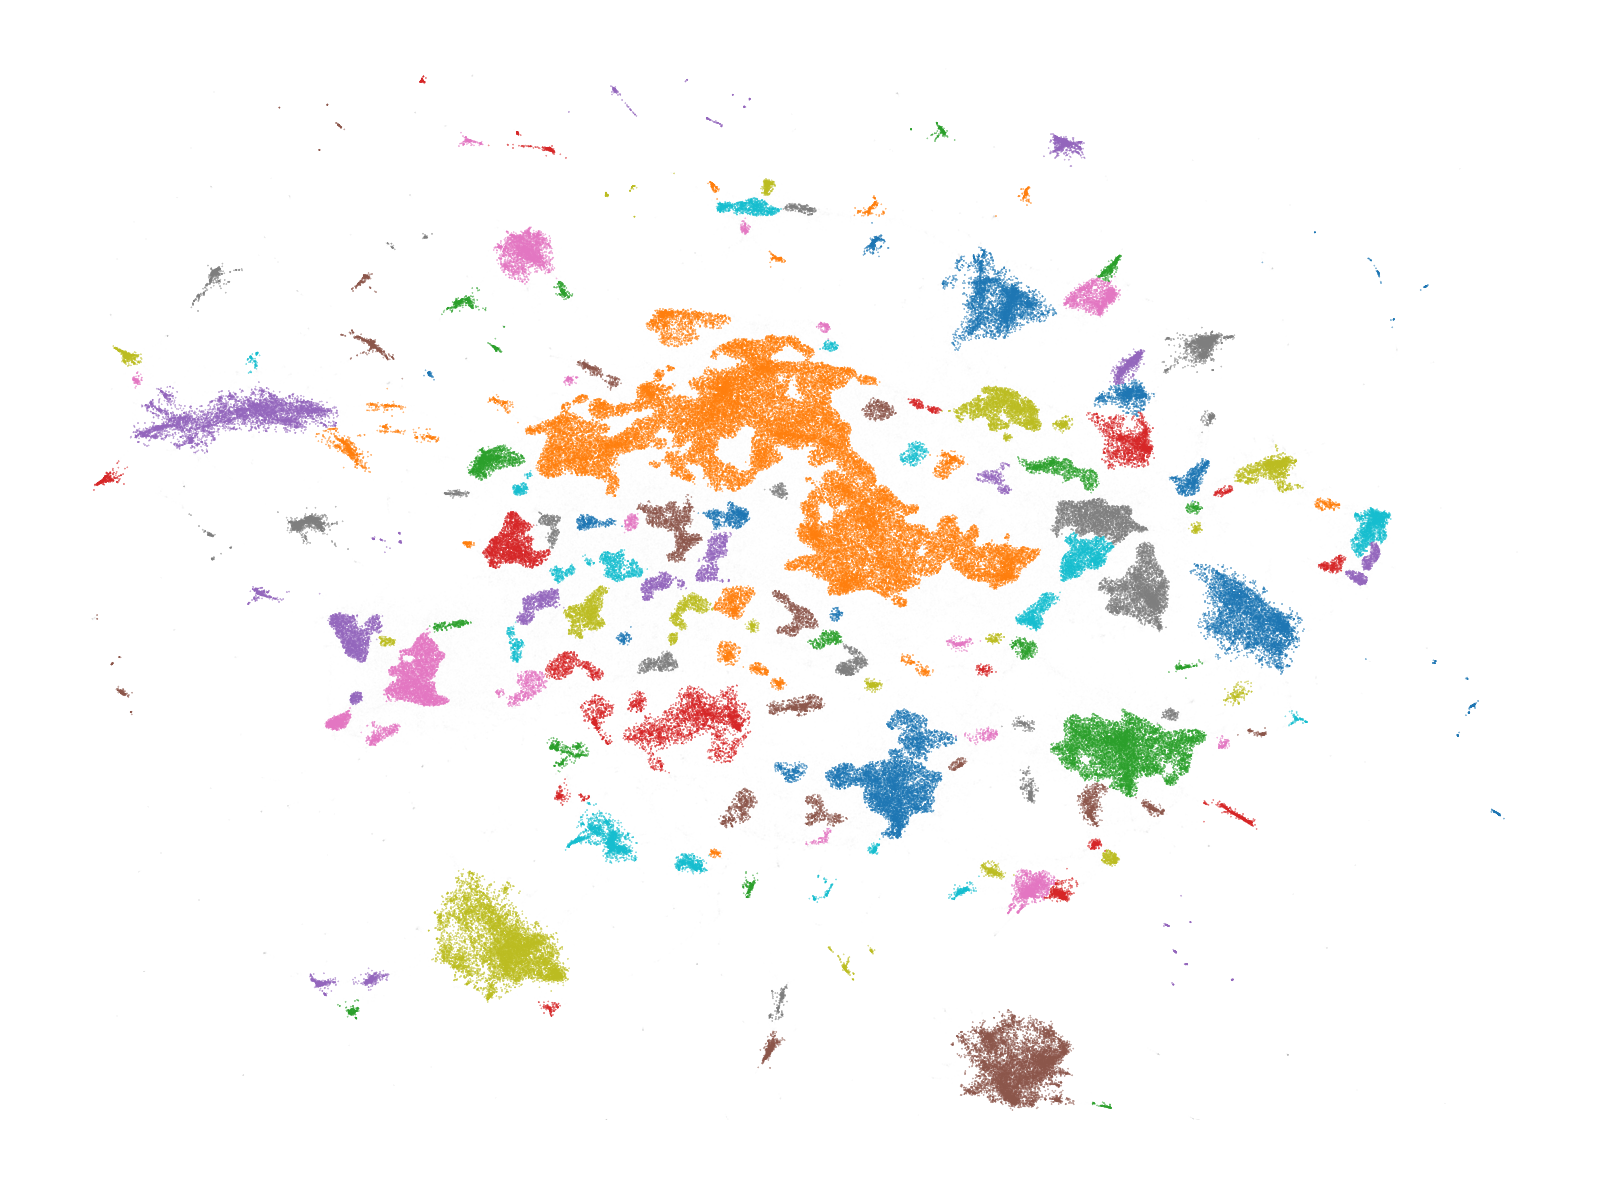
\includegraphics[width=\linewidth]{rys04/umap_5_100_100.png}
			n\_neighbors = 5
		\end{minipage}%
		\begin{minipage}{.33\textwidth}
			b)\par\medskip % chktex 10
			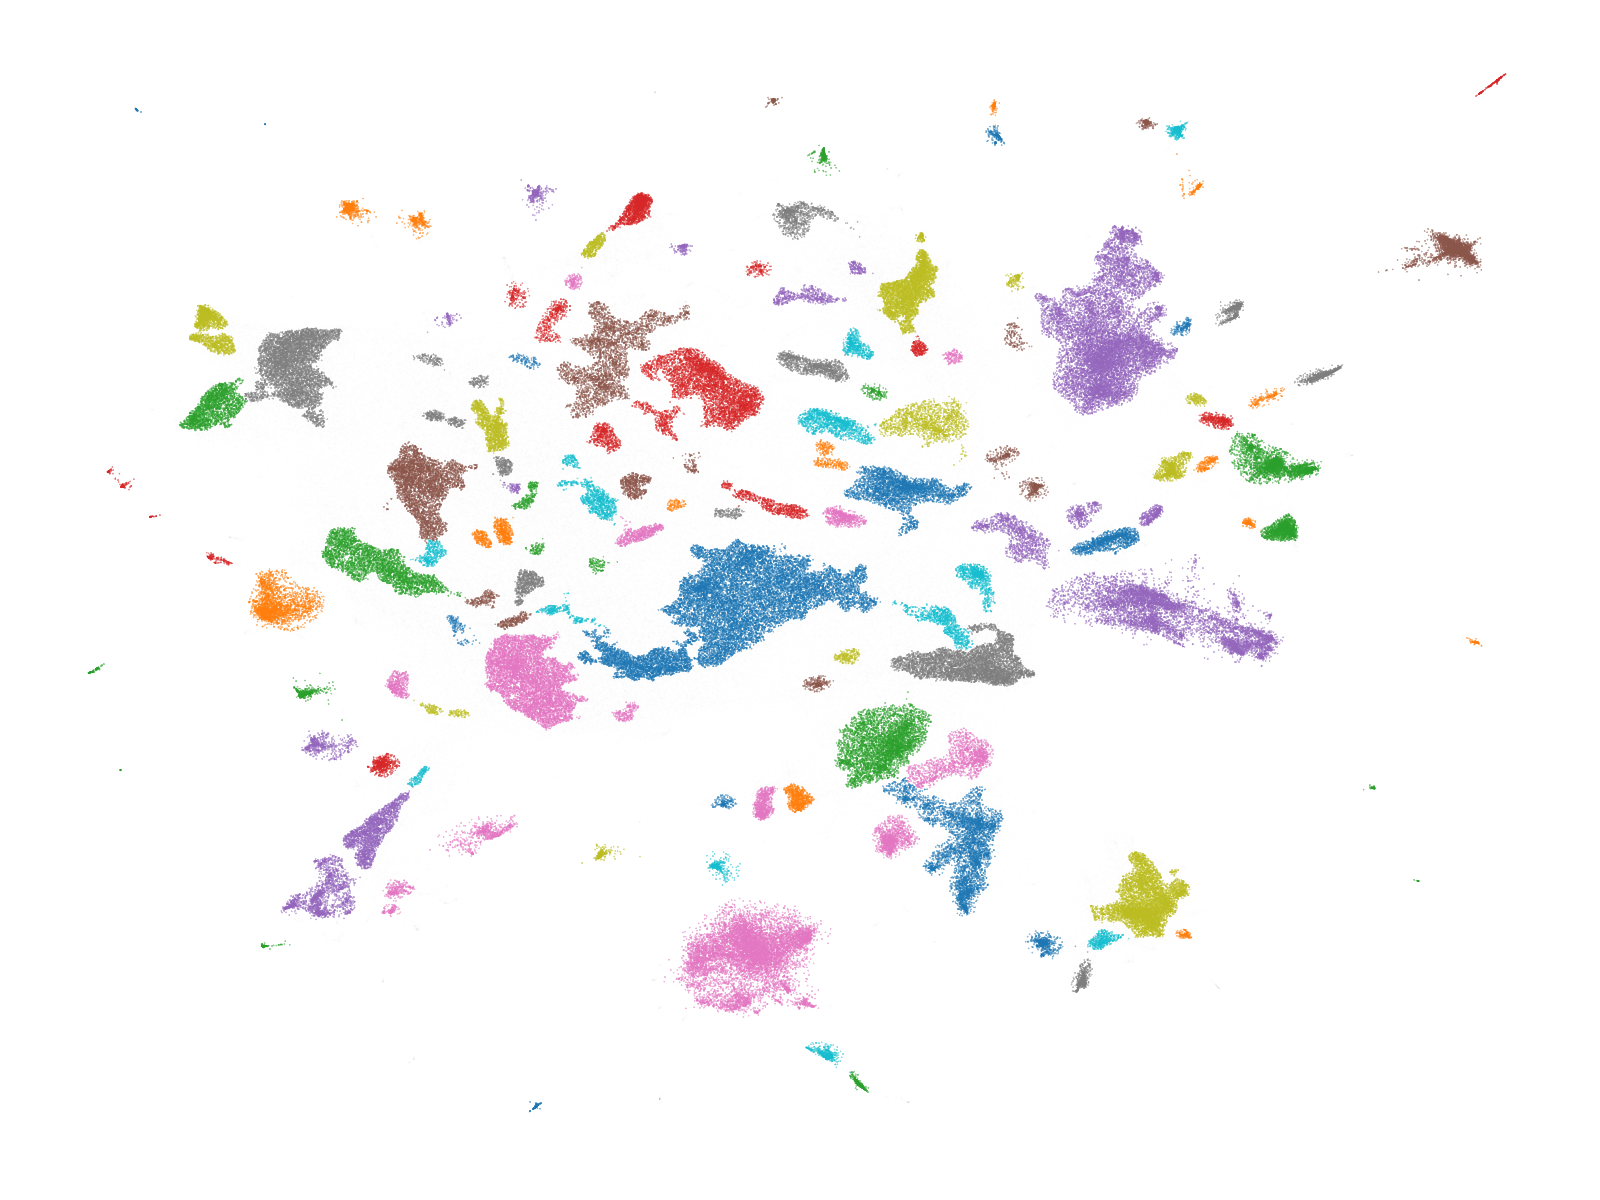
\includegraphics[width=\linewidth]{rys04/umap_15_100_100.png}
			n\_neighbors = 15
		\end{minipage}%
		\begin{minipage}{.33\textwidth}
			c)\par\medskip % chktex 10
			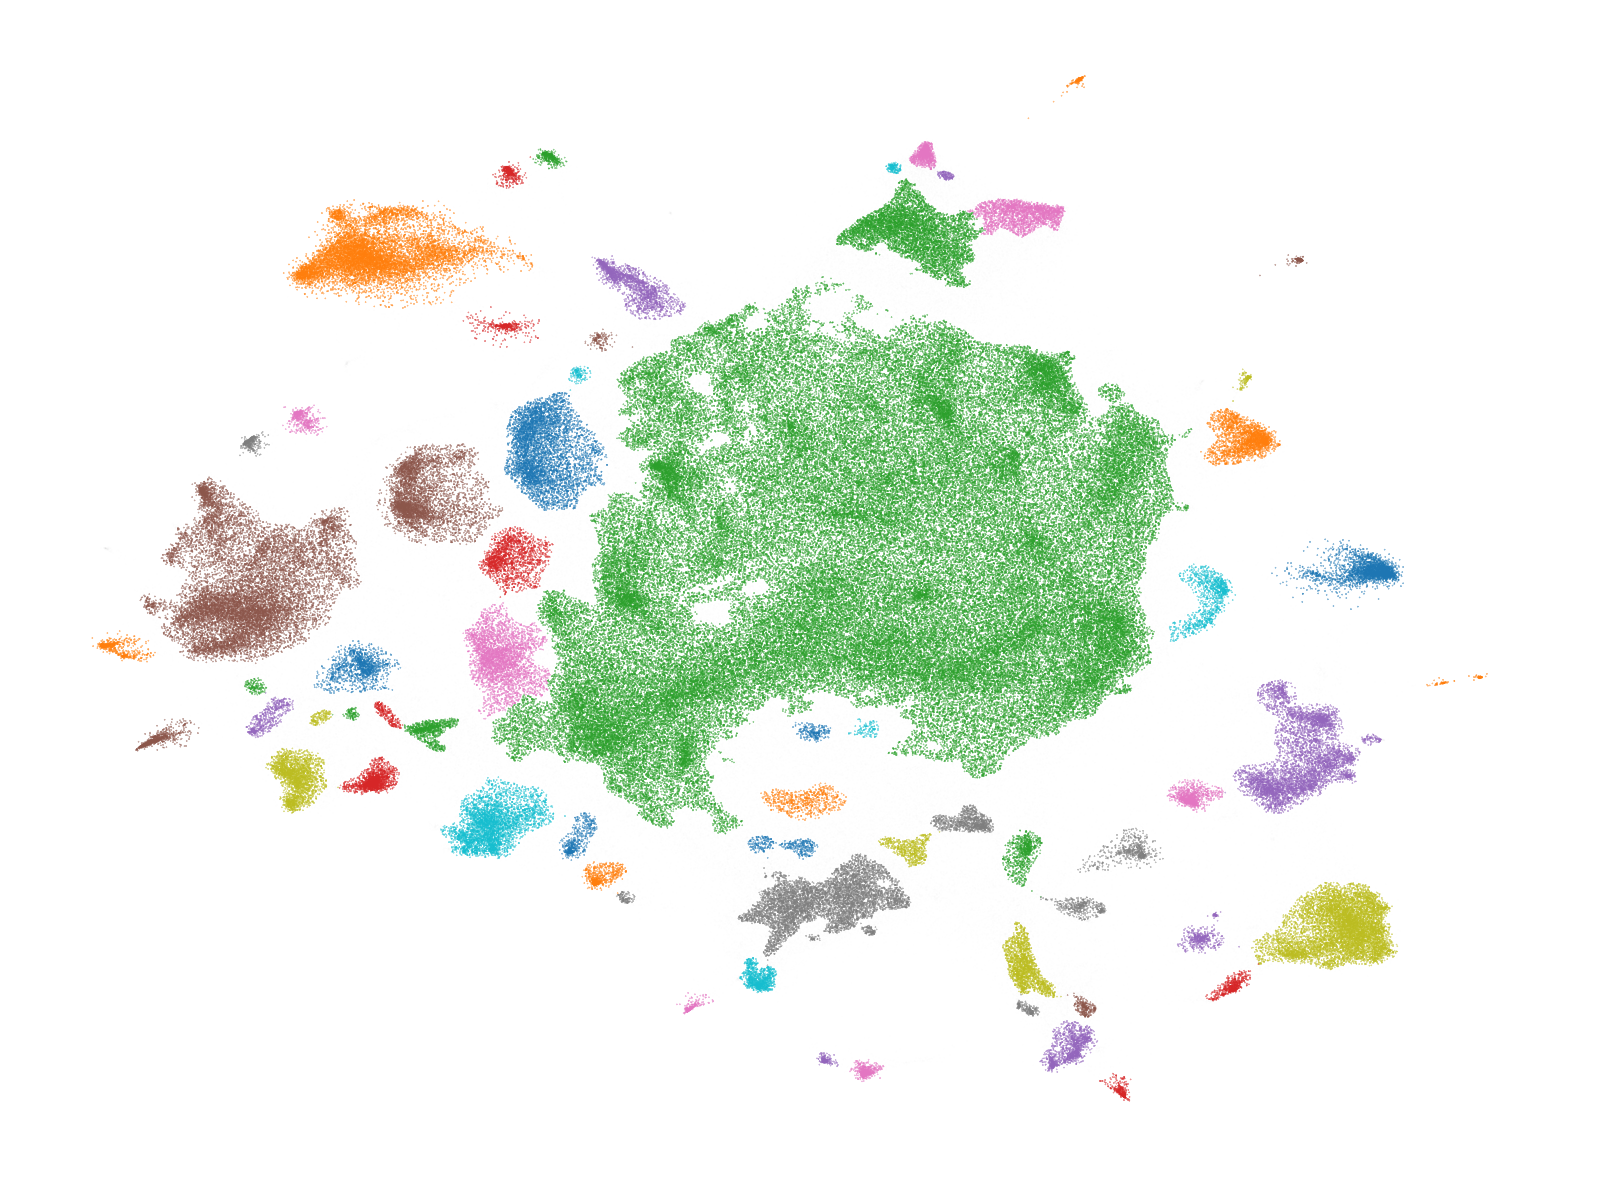
\includegraphics[width=\linewidth]{rys04/umap_100_100_100.png}
			n\_neighbors = 100
		\end{minipage}
		\caption{Dwuwymiarowa reprezentacja danych przez UMAP w zależności od wartości parametru n\_neighbors}\label{fig:umap}
	\end{figure}
	

\section{Grupowanie}\label{sec:hdbscan}
	HDBSCAN to algorytm klastrowania hierarchicznego bazujący na DBSCAN (ang.\ \emph{Density-based spatial clustering of applications with noise}).
	W celu zobrazowania działania algorytmu, wybrano ograniczony podzbiór danych.
	Z klastrów wykrytych na wszystkich danych wylosowano pięć, a z każdego z nich wylosowano dziesięć wektorów.
	Dodatkowo, wybrano dziesięć losowych wektorów bez przypisanego klastra.
	W ten sposób otrzymano 60 dokumentów, które poddano ponownej analizie HDBSCAN
		(wykorzystując wektory uzyskane z redukcji wymiarów wszystkich dokumentów do 5).
	
	Algorytm określa klastry jako rejony o większej gęstości otoczone rzadziej rozmieszczonymi punktami.
	Aby określenia gęstości używana jest metryka odległości do najbliższego \emph{k}-tego sąsiada oznaczona dalej jako \(core_k(x)\).
	Na jej podstawie stworzono metrykę określającą odległość wzajemnej osiągalności (ang.\ \emph{mutual reachability distance}):
	\[ d_k(a,b) = \max \left\lbrace core_k(a),core_k(b),d(a,b) \right\rbrace \]
	gdzie:
	\begin{itemize}
		\item \(core_k(x)\) odległość do najbliższego \emph{k}-tego sąsiada,
		\item \(d(a,b)\) pierwotna metryka odległości.
	\end{itemize}
	Dzięki takiej metryce punkty które są blisko siebie pozostają w pierwotnych odległościach, natomiast rzadsze punkty są od siebie odpychane.

	Na podstawie obliczonych odległości konstruowane jest minimalne drzewo rozpinające algorytmem Prima.
	Wierzchołkami grafu są punkty danych, a wagami krawędzi obliczone odległości.
	Na rys.~\ref{fig:mst} przedstawiono powstałe drzewo dla wyselekcjonowanych danych.
	Grubość krawędzi i kolor zależy od wartości odległości, gdzie grubsze linie oznaczają mniejszą odległość.
	Punkty pokolorowane są zgodnie z pierwotnymi klastrami, a na czarno zaznaczone są punkty, które nie miały klastrów.
	Zgodnie z oczekiwaniami, punkty nieprzypisane pierwotnie do żadnego klastra mają znacznie większe odległości od punktów, które tworzą zbiory.
	Widać też, że klastry nie nachodzą na siebie, a więc dane są dobrze odseparowane.
	
	\begin{figure}[htb]
		\centering
		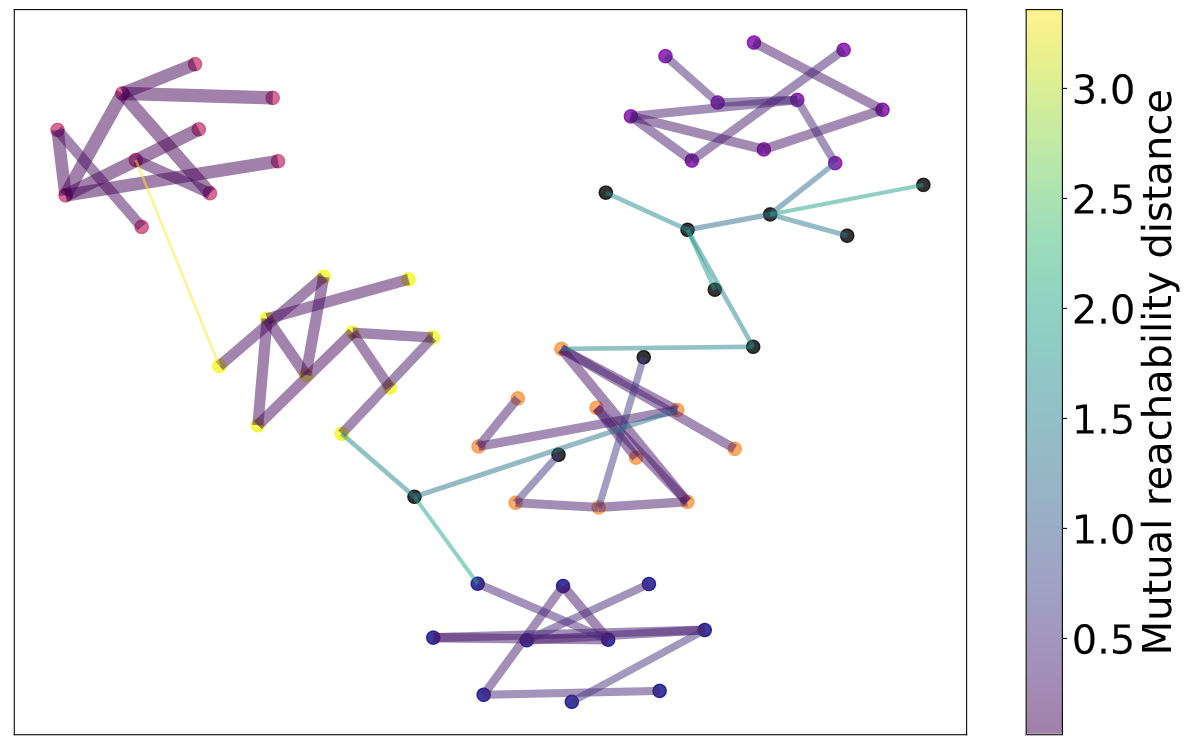
\includegraphics[width=0.5\linewidth]{rys04/hdbscan_mst.png}
		\caption{Minimalne drzewo rozpinające}\label{fig:mst}
	\end{figure}
	
	Następnie powstałe krawędzie łączone są w hierarchiczne grupy, poprzez scalanie kolejnych krawędzi o najmniejszej odległości.
	Powstałą w ten sposób hierarchię klastrów można zobrazować jako dendrogram (rys.~\ref{fig:dendrogram}a).
	Celem algorytmu jest jednak otrzymanie zbioru klastrów, nie hierarchii.
	W tym celu HDBSCAN kondensuje hierarchię do mniejszego drzewa.
	Algorytm analizuje hierarchię i podczas każdego podziału sprawdza powstałe dwie grupy.
	Jeśli obie grupy mają rozmiar większy niż minimalny (minimalny rozmiar klastra to parametr algorytmu),
		to taki podział jest traktowany jako faktyczne dwie grupy.
	Jeśli jednak któraś z powstałych grup ma mniejszy rozmiar niż minimalny to uznaje się,
		że są to punkty wypadające z klastra niestanowiące osobnej grupy i zostawiana jest jedynie większa grupa.
	W ten sposób otrzymuje się dużo mniej grup, które wraz ze wzrostem odległości między punktami zmniejszają swój rozmiar.
	Wynik takiego działania przedstawiony jest na rysunku~\ref{fig:dendrogram}b.
	
	\begin{figure}[htb]
		\centering
		\begin{minipage}{.5\textwidth}
			a)\par\medskip % chktex 10
			\begin{flushleft}
				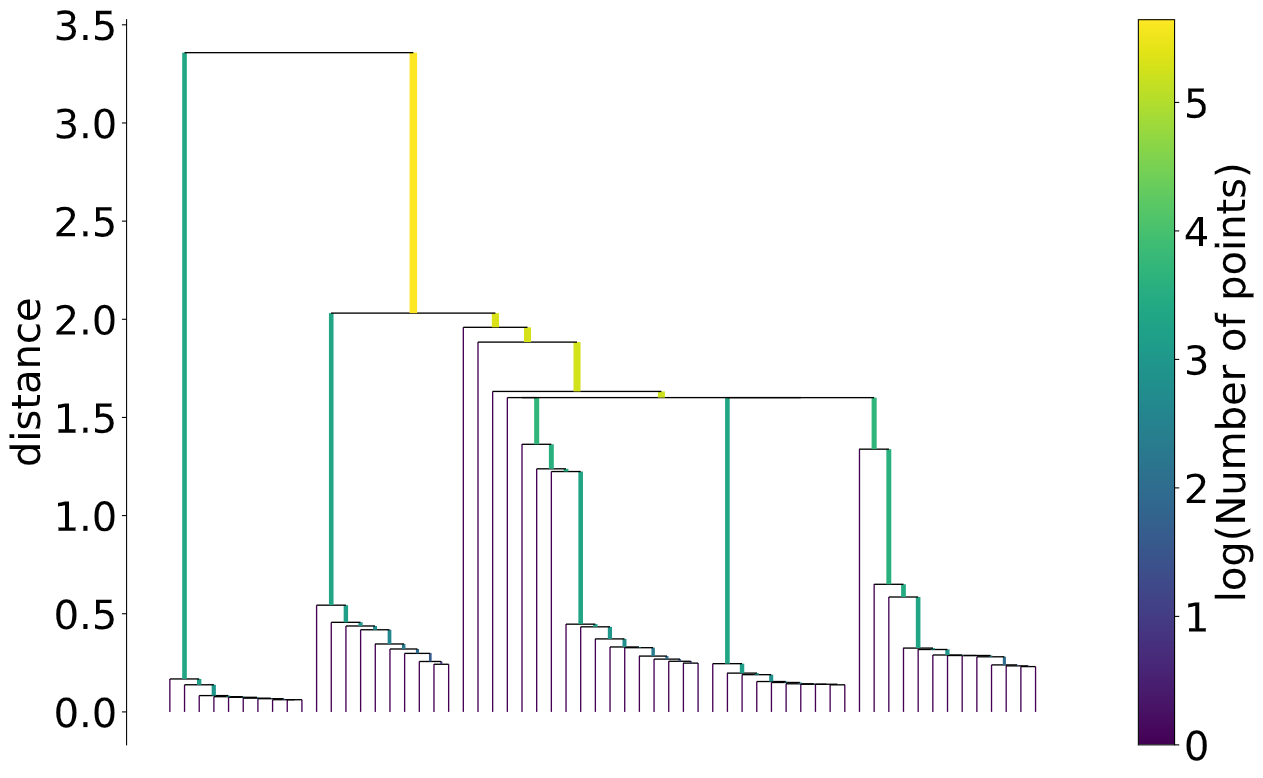
\includegraphics[width=.95\linewidth]{rys04/hdbscan_slt.png}
			\end{flushleft}
		\end{minipage}%
		\begin{minipage}{.5\textwidth}
			b)\par\medskip % chktex 10
			\begin{flushright}
				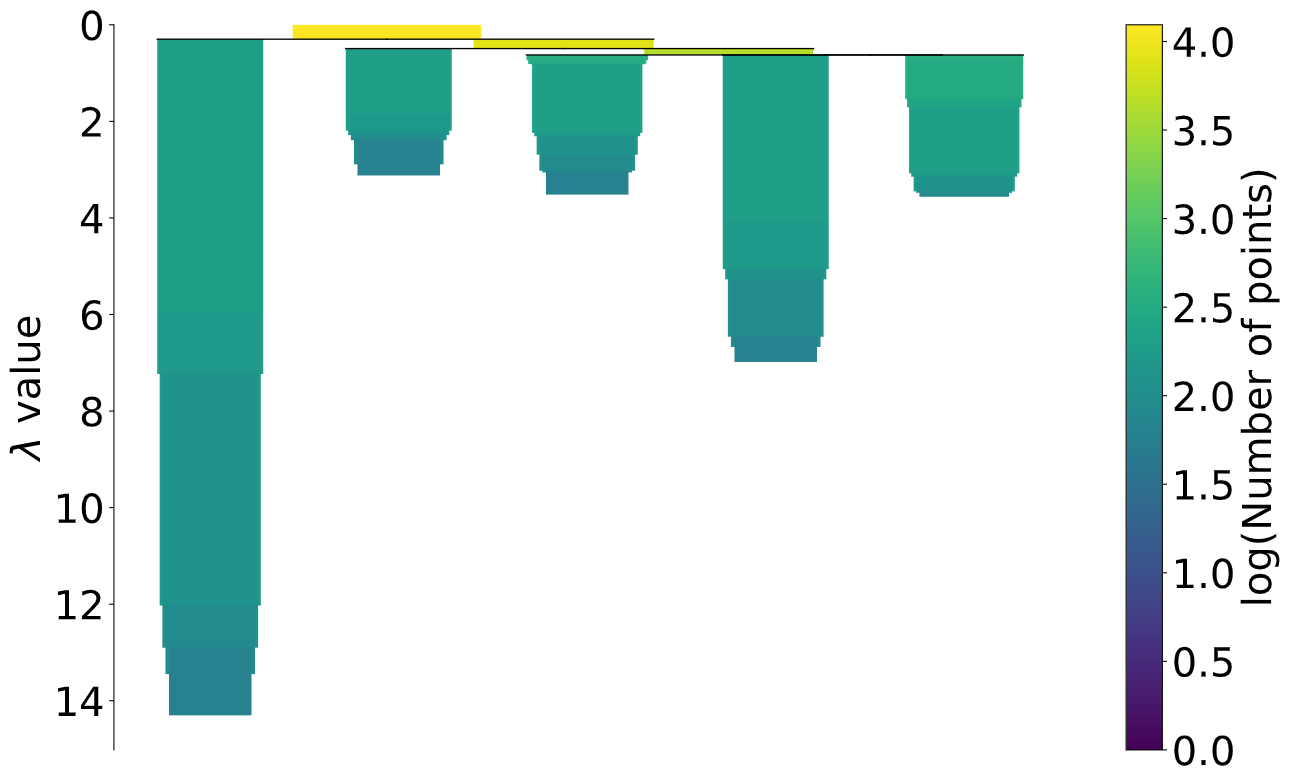
\includegraphics[width=.95\linewidth]{rys04/hdbscan_ct.png}
			\end{flushright}
		\end{minipage}
		\caption{Dendrogramy hierarchii klastrów: a) na podstawie drzewa rozpinającego, b) skondensowane}\label{fig:dendrogram} % chktex 9 chktex 10
	\end{figure}

	Na końcu z powstałego skondensowanego drzewa wybierane są najstabilniejsze klastry.
	Stabilność klastra określona na podstawie wartości \(\lambda=\frac{1}{distance}\).
	Dla każdego klastra możemy oznaczyć \(\lambda_{birth}\) i \(\lambda_{death}\) jako wartości \(\lambda\)
		odpowiednio w momencie powstania klastra i rozbicia na mniejsze klastry.
	Dla każdego punktu \(p\) w klastrze, możemy zdefiniować \(\lambda_p\)
		jako wartość \(\lambda\) w momencie, w którym punkt odłączył się od klastra, gdzie \(\lambda_{birth} < \lambda_p < \lambda_{death}\).
	Następnie dla klastra obliczamy jego stabilność jako:
	\[ \sum_{p\in cluster}\left(\lambda_p - \lambda_{birth}\right) \]

	Aby wybrać końcowe klastry najpierw zaznaczane są wszystkie liście drzewa.
	Jeśli suma stabilności dwóch łączących się klastrów jest większa niż stabilność powstałego klastra, 
		to ustawiamy stabilność klastra na tą sumę.
	Natomiast jeśli stabilność złączonego klastra jest większa niż jego potomków, to wybieramy ten klaster i odznaczamy wszystkich potomków.
	W ten sposób zaznaczamy kolejne klastry aż dojdziemy do korzenia drzewa, a powstałe zaznaczenie to zbiór klastrów.
	Na rysunku~\ref{fig:dendrogram}b zaznaczonych zostałoby pięć klastrów w kolorze morskim.
	Pozostałe punkty nienależące do tych klastrów uznawane są za szum i nie mają przypisanych grup.

	Parametr \emph{k} w implementacji algorytmu HDBSCAN nazwany jest \verb|min_samples| 
		i domyślnie jego wartość jest równa wartości \verb|min_cluster_size|.
	Na rysunku~\ref{fig:umap} wartość ta była równa 100.
	Zmniejszenie wartości \verb|min_samples| do 1 skutkuje wykryciem większej ilości mniejszych grup.
	Rezultat przedstawiony został na rys.~\ref{fig:hdbscan}a.

	Rys~\ref{fig:hdbscan}b przedstawia klastry wykryte na pięciowymiarowych wektorach, a następnie zwizualizowane na dwóch.
	Wykrywanie klastrów w przestrzeni pięciowymiarowej pozwala na dokładniejsze wykrycie zależności między punktami danych,
		które mogą zostać utracone przy redukcji do zbyt małej liczby wymiarów.
	W szczególności, punkty oznaczone jako szum w pięciu wymiarach, w dwóch wymiarach wykrywane są jako klastry.
	
	\begin{figure}[htb]
		\centering
		\begin{minipage}{.5\textwidth}
			a)\par\medskip % chktex 10
			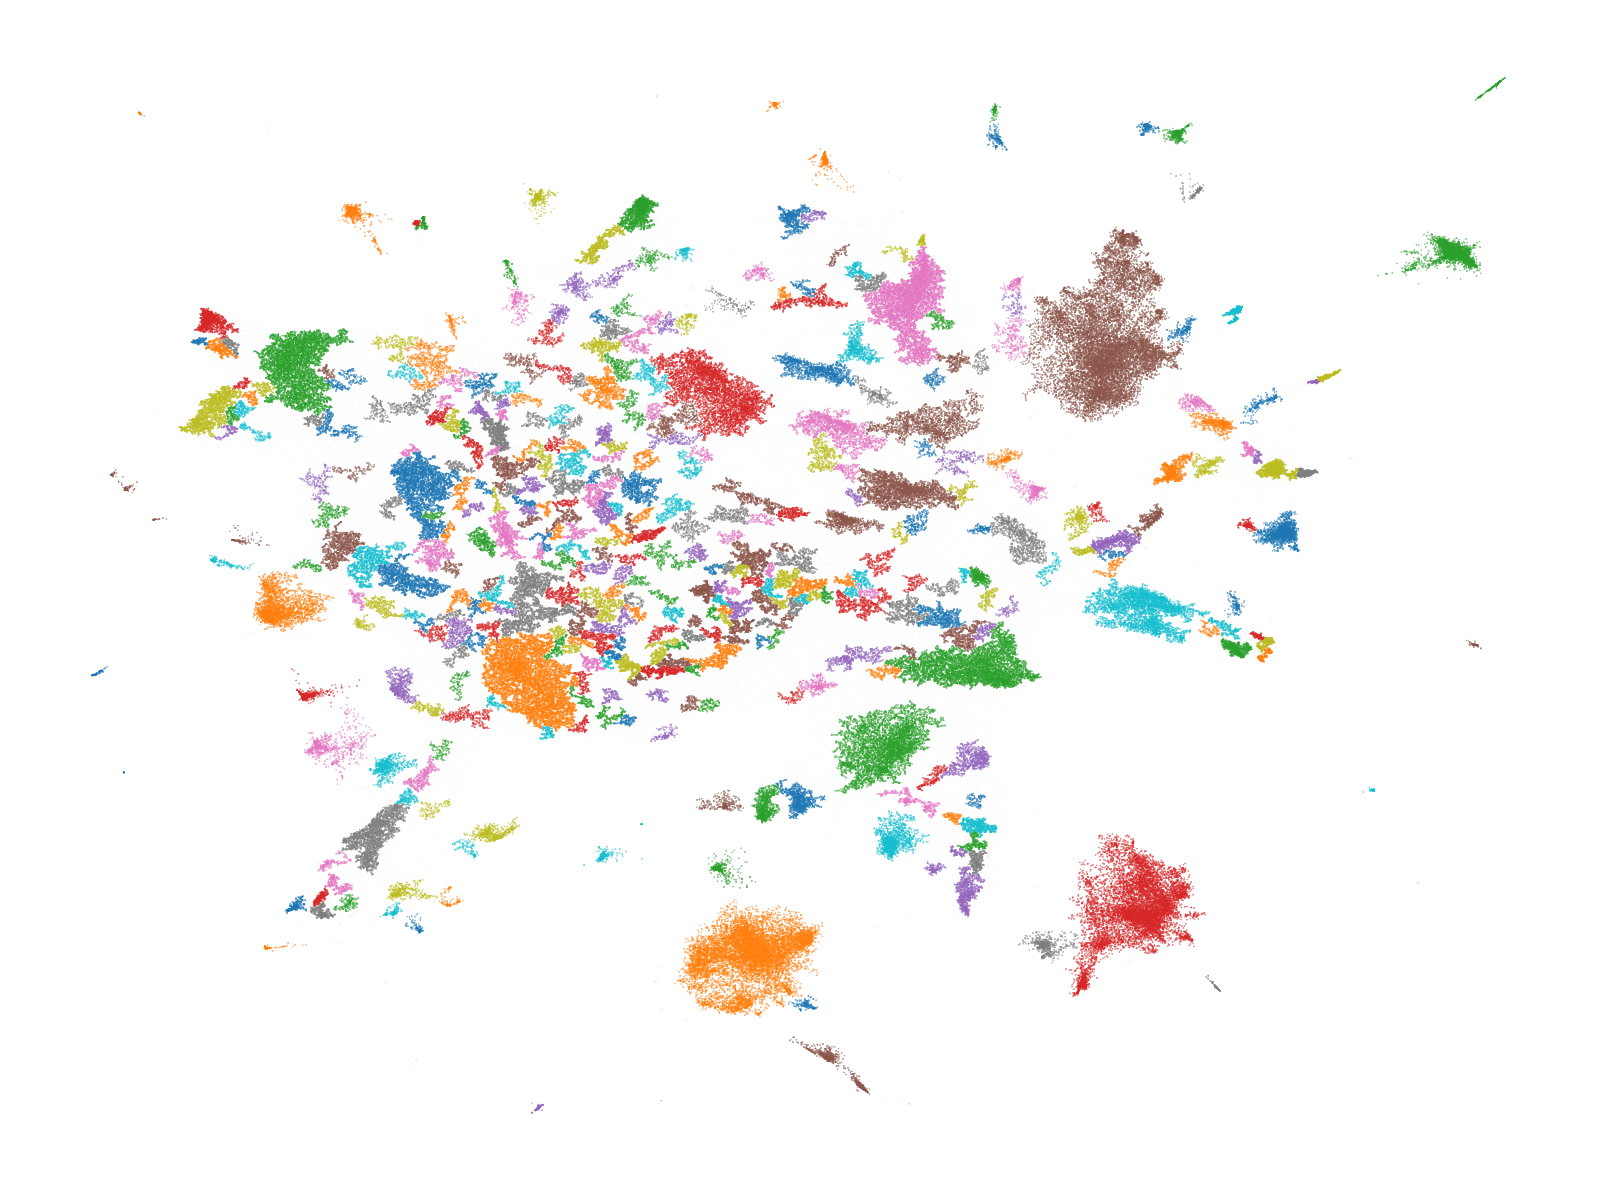
\includegraphics[width=\linewidth]{rys04/umap_15_100_1.png}
		\end{minipage}%
		\begin{minipage}{.5\textwidth}
			b)\par\medskip % chktex 10
			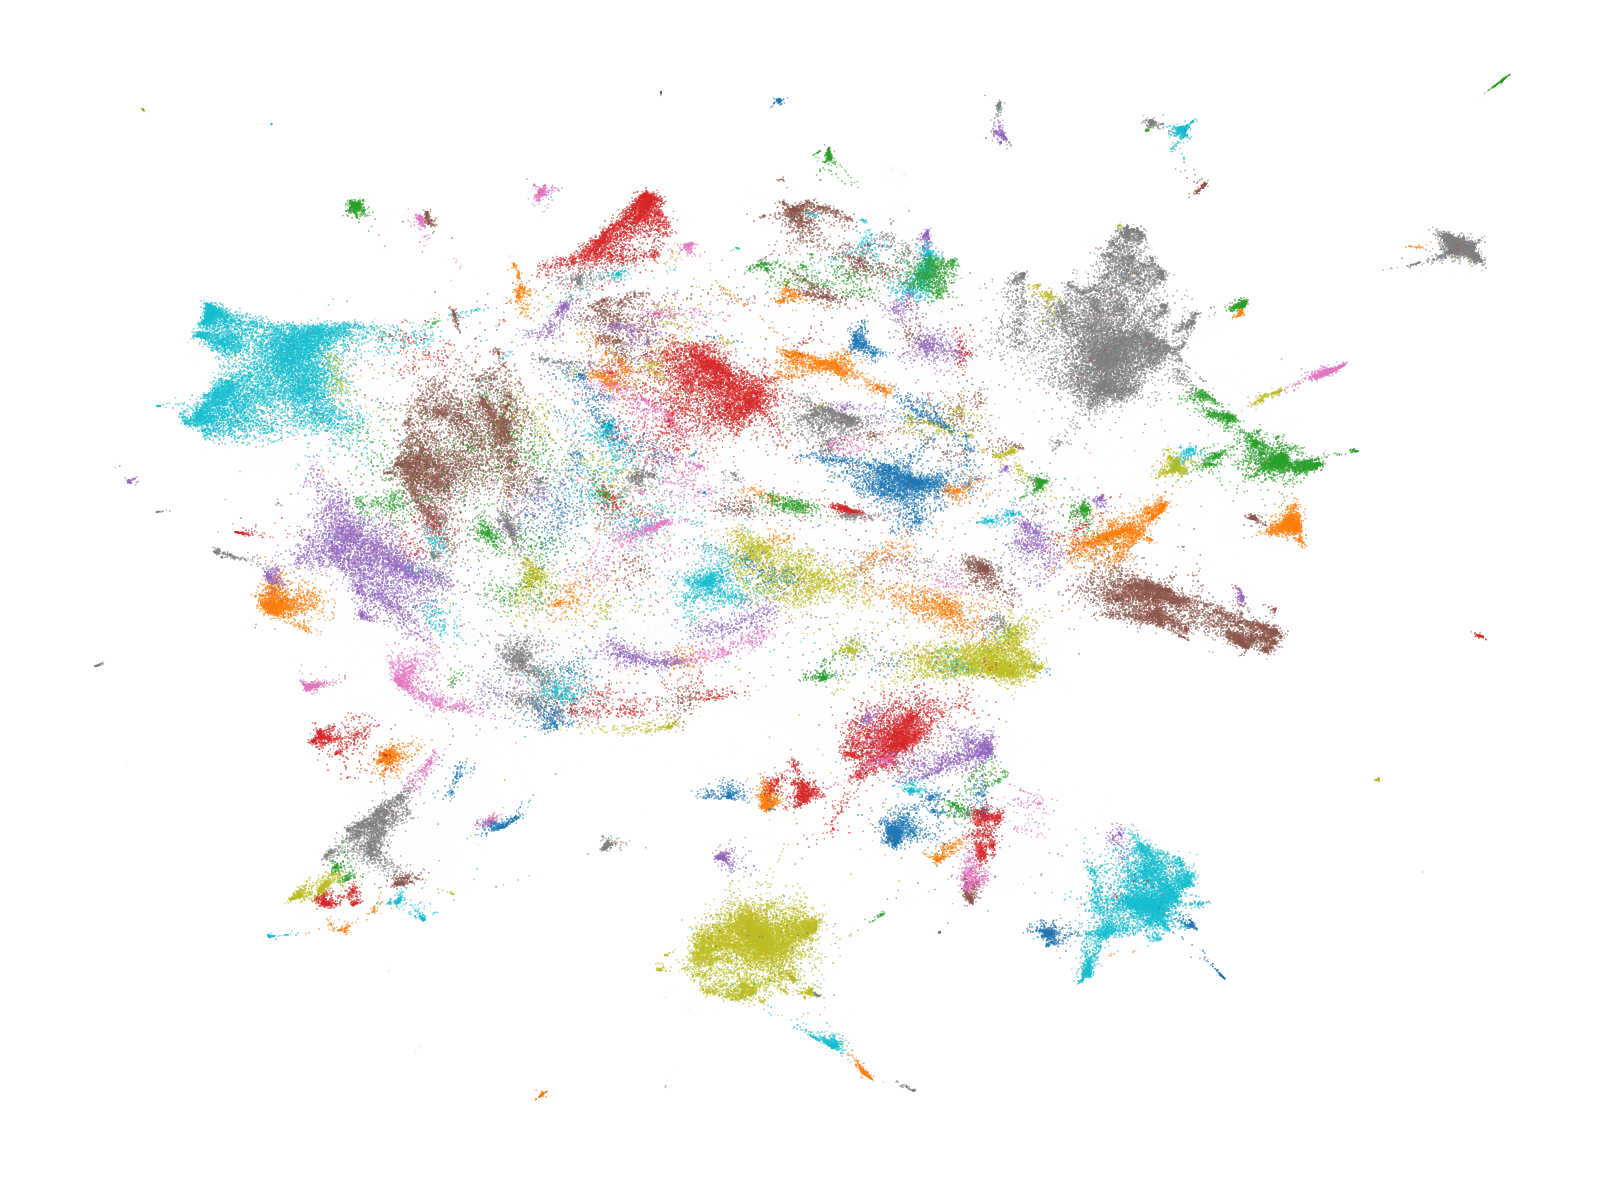
\includegraphics[width=\linewidth]{rys04/umap_15_100_1_5d.png}
		\end{minipage}
		\caption{Wykryte klastry na wektorach: a) dwuwymiarowych, b) pięciowymiarowych}\label{fig:hdbscan} % chktex 9 chktex 10
	\end{figure}

\section{Reprezentacja tematu}
	Każdy temat reprezentowany jest zbiorem słów najlepiej opisujących zawarte w nim dokumenty.
	Jednocześnie słowa te powinny być specyficzne dla danego zbioru tak, aby widoczne były różnice między tematami.
	Jest to problem podobny do wyszukiwania słów identyfikujących dokument algorytmem TF-IDF\@.
	Tym razem jednak chcemy znaleźć słowa identyfikujące zbiór dokumentów na tle innych zbiorów.
	Autor BERTopic nazwał tą wariację algorytmu c-TF-IDF (ang.\ \emph{class-based TF-IDF}):
	\[c-TF-IDF_i = \frac{t_i}{w_i} \cdot \log \frac{m}{\sum_j^n t_j} \]
	gdzie:
	\begin{itemize}
		\item \(t_i\) częstość występowania słowa \emph{t} w klasie \emph{i},
		\item \(w_i\) liczba słów w klasie \emph{i},
		\item \(m\) liczba wszystkich pierwotnych dokumentów (niezgrupowanych),
		\item \(\sum_j^n t_j\) suma częstości występowania słowa \emph{t} we wszystkich klasach.
	\end{itemize}

	W ten sposób uzyskano ranking wszystkich słów w danej klasie.
	Na podstawie tego rankingu wybiera się 5--10 słów z najwyższym wynikiem, które stanowią reprezentację tematu.
	Często zdarza się jednak, że otrzymane słowa będą bardzo podobne.
	Przykładowe reprezentacje powstałe tą metodą przedstawione zostały w tabeli~\ref{tab:mmr}.
	Aby zminimalizować liczbę podobnych słów w reprezentacji tematu i jednocześnie zdywersyfikować opis tematu,
		w BERTopic zastosowany jest algorytm MMR (ang.\ \emph{Maximal Marginal Relevance})\cite{MMR}:
	\[MMR = \arg \max_{D_i \in R\backslash S} \left[\lambda\left(Sim_1(D_1, Q) - (1-\lambda) \max_{D_j \in S} Sim_2(D_i, D_j)\right)\right]\]
	gdzie:
	\begin{itemize}
		\item \(D_i\) analizowany kandydat,
		\item \(R\backslash S\) zbiór kandydatów, bez już wybranych,
		\item \(\lambda\) stała w zakresie \(\left[0,1\right]\), kontrolująca zróżnicowanie wyników (0 dla maksymalnie zdywersyfikowanych, 1 dla listy odpowiadającej wzięciu wprost najlepszych wyników),
		\item \(S\) zbiór już wybranych kandydatów,
		\item \(Q\) zapytanie,
		\item \(Sim_1\) metryka podobieństwa kandydata do zapytania,
		\item \(Sim_2\) metryka podobieństwa kandydatów między sobą.
	\end{itemize}
	W kontekście poszukiwania najlepszej reprezentacji tematu, kandydatami są słowa z najwyższymi wynikami \emph{c-TF-IDF}, a zapytanie to wektor całego tematu.
	Wektor tematu obliczany jest wybranym modelem SBERT kodującym dokument powstały z połączenia trzydziestu słów tematu o najwyższych wynikach \emph{c-TF-IDF}.
	Natomiast jako obie metryki \(Sim_1\) i \(Sim_2\) wykorzystywane jest podobieństwo kosinusowe.
	Wartość parametru \(\lambda\) ustawiono na 0 (maksymalna dywersyfikacja).
	W ten sposób otrzymuje się reprezentacje tematów dużo lepiej opisujące zbiory,
		co jest szczególnie istotne w języku polskim zawierającym wiele odmian tych samych słów.
	Tabela~\ref{tab:mmr} przedstawia reprezentacje tematów otrzymane po zastosowaniu MMR\@.

	\begin{table}[htb]
		\caption{Reprezentacje wybranych tematów: a) bez MMR, b) z MMR}\label{tab:mmr} % chktex 9 chktex 10
		\centering
		a) % chktex 10
		\begin{tabularx}{.9\textwidth}{rl}
			\toprule
			A	&	morskich | statków | morskiego | statku | morskiej	\\ 
			B	&	lotnicze | lotnictwa | lotniczego | lotnisk | lotniczych	\\ 
			C	&	celnego | celnych | towarów | celne | celny	\\
			\midrule
		\end{tabularx}

		b) % chktex 10
		\begin{tabularx}{.9\textwidth}{rl}
			A	&	statków | statkach | marynarzy | gospodarki morskiej | administracji morskiej	\\ 
			B	&	lotnicze | lotnictwa | lotnictwa cywilnego | prawo lotnicze | ruchu lotniczego \\ 
			C	&	celnego | celnych | prawo celne | kodeks celny | prawa celnego \\
			\bottomrule
		\end{tabularx}
	\end{table}